\documentclass[12pt, a4paper, oneside]{article}
\usepackage{astronotes}

\begin{document}

\pagestyle{fancy}
\fancyhf{}
\lhead{\textbf{กิตติพัศ พงศ์อรุโณทัย}\\{\today}}
\rhead{\textbf{ReadMe\_01}\\Welcome to AstroNotes}
\cfoot{\thepage}

\begin{titlepage}
    \centering
    
    %
\includegraphics[width=0.15\textwidth]{img/sklogo.png}
    %
\includegraphics[width=0.15\textwidth]{img/kvislogo.png}
    %
\includegraphics[width=0.15\textwidth]{img/mwitlogo.png}
    %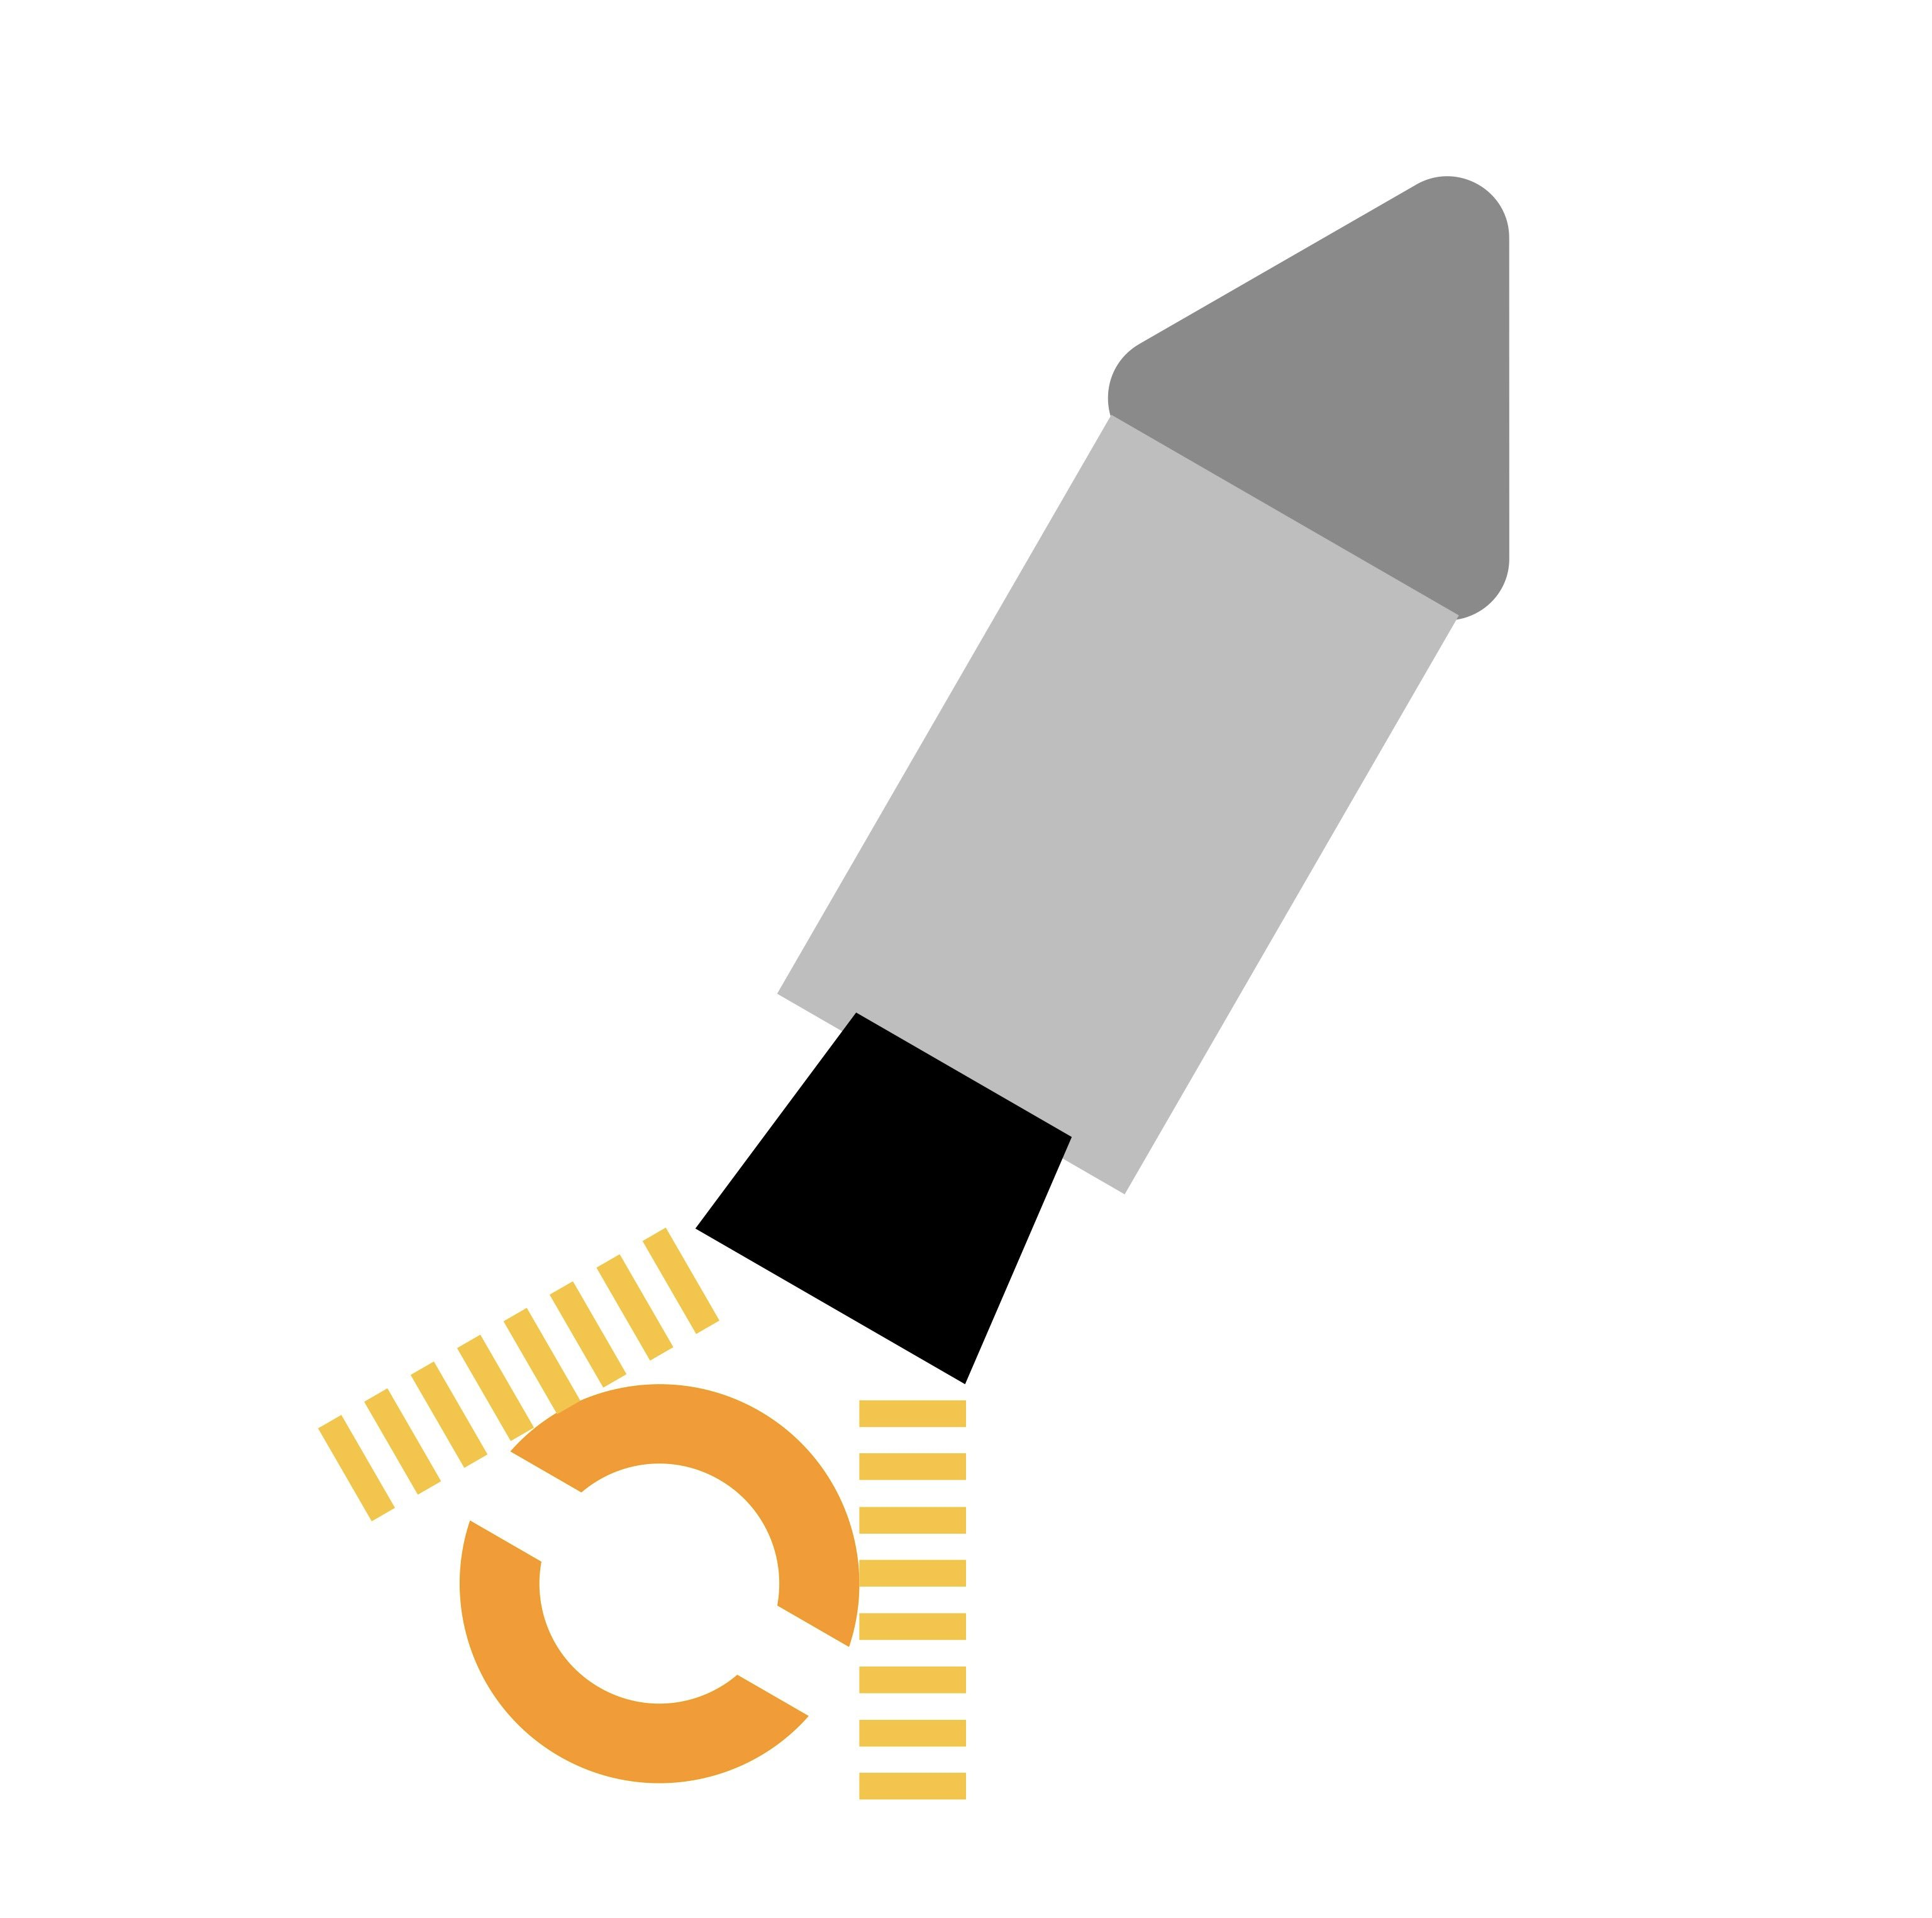
\includegraphics[width=0.15\textwidth]{img/mzpfp1.jpg}
    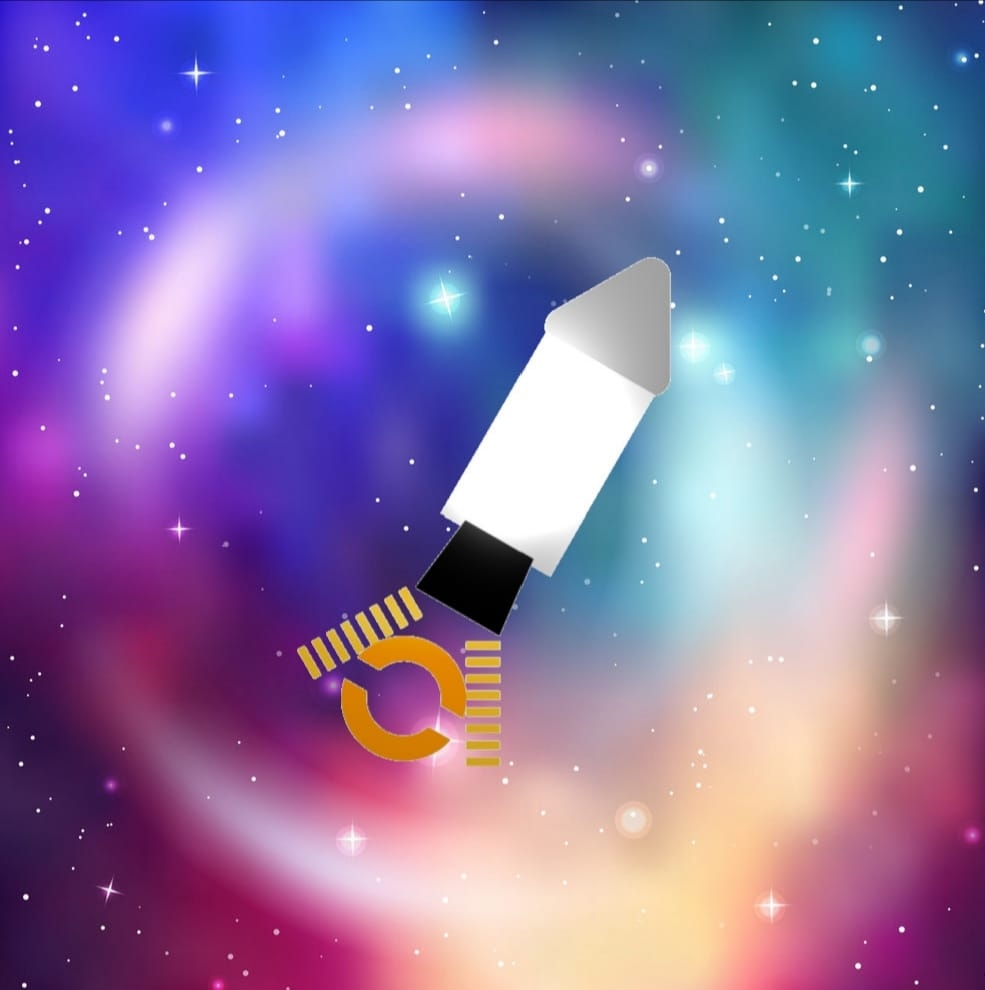
\includegraphics[width=0.15\textwidth]{img/mzpfp2.jpg}
    \par\vspace{1cm}
	{\Large \textsc{Astronomy POSN Summaries (AstroNotes)}\par}
    \vspace{0.25cm}
	{\Large \textsc{ไฟล์สรุปสำหรับ สอวน. ดาราศาสตร์}\par}

	\vspace{2cm}
	{\LARGE\bfseries Welcome to Project AstroNotes!\par}
    \vspace{0.25cm}
    {\LARGE\bfseries ยินดีต้อนรับสู่ AstroNotes!\par}

	\vspace{1cm}
	{\Large\itshape กิตติพัศ พงศ์อรุโณทัย\par}
    \vspace{0.25cm}
    {\large\itshape โรงเรียนกำเนิดวิทย์\par}
    {\itshape ศูนย์ สอวน. ดาราศาสตร์ โรงเรียนมหิดลวิทยานุสรณ์ และโรงเรียนสวนกุหลาบวิทยาลัย}
	\vfill
% Bottom of the page
	{\large \today\par}
\end{titlepage}

\section{ยินดีต้อนรับสู่ AstroNotes}
สวัสดีครับทุกคน ยินดีต้อนรับสู่โปรเจกต์ของผม ในที่นี้จะมีไฟล์สรุปเนื้อหาทางดาราศาสตร์มากมายให้เข้ามาอ่านได้ โดยมีขั้นตอนการอ่านให้อย่างสมบูรณ์
ขอขอบคุณทุกคนที่เข้ามาอ่าน AstroNotes นะครับ หวังว่าทุกคนจะได้รับอะไรจากโปรเจกต์เล็กๆ ของผมไม่มากก็น้อย

\section{ที่มาของ AstroNotes}
เคยมีคนถามผมว่า "อยากเข้า สอวน. ดาราศาสตร์ อ่านหนังสืออะไรดี" 
คำตอบที่ดีที่สุด แน่นอนคือ Fundamental Astronomy ของ Karttunen\cite{karttunen2007fundamental} แต่คำตอบกลับมาตลอดว่า "อ่านภาษาอังกฤษไม่รู้เรื่องอ่ะพี่"\\
เป็นปัญหาอยู่นาน สอวน. ก็ไม่มีหนังสือซะด้วย หนังสืออื่นๆ ก็ยากไป ไม่ก็ไม่เหมาะกับ สอวน. ซักเท่าไร สุดท้ายผมก็ตัดสินใจเขียนหนังสือ แต่มันก็เยอะไป เลยลองแยกไฟล์ออกมา ทำปก แล้วมันดันสวยแล้วอ่านได้\\
AstroNotes ก็เลยถือกำเนิดขึ้นมาครับ


\section{ขอบเขตของ AstroNotes}
สิ่งที่ควรรู้ก่อนเริ่มอ่าน AstroNotes ก็คือเนื้อหาฟิสิกส์ และคณิตศาสตร์ ม.ต้นทั้งหมด กล่าวคือ
\begin{enumerate}
    \item การแก้สมการ (1,2 ตัวแปร และกำลังสอง)
    \item ตรีโกณมิติ
    \item ฟังค์ชั่น (พหุนาม, ตรีโกณมิติ, Exponential และ Inverse)
    \item กลศาสตร์ (การเคลื่อนที่ 1,2 มิติและวงกลม)
    \item งาน พลังงานและโมเมนตัม (ปกติและเชิงมุม)
\end{enumerate}
เนื้อหาทั้งหมด จะรวมตั้งแต่\textbf{เนื้อหาปูพื้นฐาน} เช่นแคลคูลัส เวกเตอร์ \textbf{เนื้อหาค่าย 1} เช่นกฎของเคปเลอร์ กฎของสเตฟาน-โบลซ์แมน \textbf{เนื้อหาค่าย 2} เช่นจุดลากรานจ์ สมดุลสถิตย์ในดาว \textbf{เนื้อหา IOAA} เช่นสมการของฟรีดแมน ทฤษฎีสัมพัทธภาพพิเศษ และ\textbf{เนื้อหาที่มีความน่าสนใจ} เช่นกลศาสตร์ลากรานจ์ การเขียน LaTeX โดยในบางครั้ง หากเนื้อหาที่น่าสนใจช่วยในการเข้าใจเนื้อหาอื่นๆ อาจเป็น Prerequisite ได้

\section{ประกาศกิตติคุณ (Dedications)}
โปรเจกต์นี้ เป็นโปรเจกต์ที่เกิดจากความตั้งใจของตัวผมเอง อย่างไรก็ตาม กว่าผมจะมีความรู้มากพอจะทำโปรเจคนี้ได้ มีคนมากมายที่มีส่วนในการทำให้ผมมีวันนี้
\begin{enumerate}
    \item ศูนย์ สอวน. ดาราศาสตร์ โรงเรียนมหิดลวิทยานุสรณ์ และโรงเรียนสวนกุหลาบวิทยาลัย ร่วมถึงรุ่นพี่ รุ่นน้อง อาจารย์ทุกท่าน ที่ช่วยสอนผมจากตอนผมยังคงเป็นเด็กธรรมดา
    \item อาจารย์ค่ายผู้แทนประเทศทุกท่านและอาจารย์อีกหลายท่านที่ไม่ได้เอ่ยนาม ที่ช่วยเตรียมผมในการเข้าแข่งขัน
    \item มูลนิธิสอวน. ที่ให้โอกาสนักเรียนทั่วประเทศในการเรียนรู้
    \item เพื่อนๆ กำเนิดวิทย์และสวนกุหลาบ ที่ให้การสนับสนุนที่ดีเสมอมา
    \item ครอบครัวผม ที่ดูแลผม โดยเฉพาะพ่อและแม่ ที่ทำให้ผมได้ลืมตามาดูเอกภพที่สวยงามนี้
\end{enumerate}

\section{ปัจฉิมลิขิต (Ending Remarks)}
เส้นทางแห่งดาราศาสตร์นั้นยาวไกล ขอให้ทุกคนมีกำลังใจและมุ่งมั่น อย่างน้อยหากไม่ได้เป็นผู้แทนศูนย์หรือผู้แทนประเทศ เราก็ได้ความรู้และได้หลงไหลในจักรวาล ขอให้โชคดีครับ
\bibliographystyle{ieeetr}
\bibliography{bibliography}
\end{document}
